\documentclass[12pt]{article}

\usepackage[a4paper, margin=1in]{geometry}
\usepackage{fancyhdr}
\usepackage{lastpage}
\usepackage{amsmath}
\usepackage{amsfonts}
\usepackage{tikz}
\usepackage[most]{tcolorbox}
\usepackage{amsthm}
\usepackage{etoolbox}
\usepackage{amssymb}

\setlength{\headheight}{15pt}
\pagestyle{fancy}
\fancyhf{}
\lhead{\textbf{Related Rates - Worked Examples}}
% \rhead{\textbf{SUBTITLE}}
\lfoot{\textbf{St. Francis Xavier University}}
\rfoot{\textbf{Carter Clifton}}
\renewcommand{\headrulewidth}{0.3pt}
\renewcommand{\footrulewidth}{0.3pt}

\tcbset{
    grayscalebox/.style={
        enhanced,
        sharp corners,
        colback=gray!5,
        colframe=black!10,
        boxrule=0.3pt,
        left=1em,
        right=1em,
        top=0.5em,
        bottom=0.5em,
        fonttitle=\bfseries\normalsize,
        coltitle=black,
        before skip=10pt,
        after skip=10pt
    }
}

\newtcbtheorem[no counter]{theorem}{Theorem}{grayscalebox}{th}
\newtcbtheorem[no counter]{lemma}{Lemma}{grayscalebox}{lem}
\newtcbtheorem[no counter]{corollary}{Corollary}{grayscalebox}{cor}
\newtcbtheorem[no counter]{proposition}{Proposition}{grayscalebox}{prop}
\newtcbtheorem[no counter]{definition}{Definition}{grayscalebox}{def}
\newtcbtheorem[no counter]{example}{Example}{grayscalebox}{ex}
\newtcbtheorem[no counter]{remark}{Remark}{grayscalebox}{rem}

\newcommand{\horrule}{\noindent\rule{\linewidth}{0.3pt}\newline}
\newcommand\at[2]{\left.#1\right|_{#2}}

\title{Related Rates - Worked Examples}
\author{Carter Clifton}
\date{\today}

\begin{document}

\maketitle

\newpage

\section*{Expanding Sphere}

\subsection*{Question}

Consider a spherical balloon whose \textbf{volume} is expanding at a \textbf{rate of $ \mathbf{0.5} $ cm$ \mathbf{^3} $/sec}. How fast is the \textbf{radius changing} when the \textbf{radius} is $ \mathbf{10} $ \textbf{cm}?

\subsection*{Diagram}

\begin{center}
    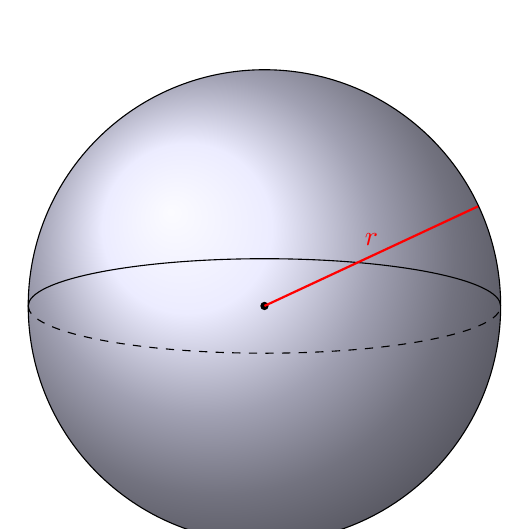
\begin{tikzpicture}
        \shade[ball color=blue!10] (0, 0) circle (3);
        \draw[dashed] (180:3) arc[start angle = 180, end angle = 360, x radius = 3, y radius = 0.6];
        \draw (0:3) arc[start angle = 0, end angle = 180, x radius = 3, y radius = 0.6];
        \fill (0, 0) circle (1.5pt);
        \draw[thick, red] (0,0) -- (25:3)
            node[midway, above] {$ r $};
        \draw (0, 0) circle (3);
    \end{tikzpicture}
\end{center}

\subsection*{Solution}

Let $ V $ = volume of the balloon, $ r $ = radius of the balloon, and $ t $ = time.
\medskip
\newline
We know $ \frac{dV}{dt} = 0.5 $ cm$ ^3 $/sec, and we want to find $ \frac{dr}{dt} $ when $ r = 10 $ cm. Using the chain rule, we can write:
\[ \frac{dV}{dt} = \frac{dV}{dr} \cdot \frac{dr}{dt} \]
Also, note that the volume of a sphere is given by:
\[ V = \frac{4}{3} \pi r^3 \]
Using this equation for the volume, we can differentiate to find $ \frac{dV}{dr} $.
\begin{align*}
    \frac{dV}{dr} & = \frac{d}{dr} \left( \frac{4}{3} \pi r^3 \right) \\
    & = \frac{4}{3} \pi \left( 3 r^2 \right) \\
    & = 4 \pi r^2
\end{align*}
Plugging this, as well as $ \frac{dV}{dt} $, into our chain rule equation gives:
\begin{align*}
    \frac{dV}{dt} & = \frac{dV}{dr} \cdot \frac{dr}{dt} \\
    0.5 & = 4 \pi r^2 \cdot \frac{dr}{dt} \\
    \frac{dr}{dt} & = \frac{0.5}{4 \pi r^2}
\end{align*}
Now, substitute $ r = 10 $ into this expression.
\begin{align*}
    \at{\frac{dr}{dt}}{r = 10} & = \frac{0.5}{4 \pi \left( 10 \right)^2} \\
    & = \frac{0.5}{4 \pi \cdot 100} \\
    & = \frac{0.5}{400 \pi} \\
    & = \frac{1}{800 \pi} \ \text{cm/sec} \\
    & \approx 0.000398 \ \text{cm/sec} \\
    & \approx 3.98 \times 10^{-4} \ \text{cm/sec}
\end{align*}
Therefore, the radius of the balloon is changing at a rate of approximately $ 3.98 \times 10^{-4} $ cm/sec when the radius is $ 10 $ cm.

\section*{Gravel Pile}

\subsection*{Question}

Gravel falls off of a conveyor belt at a \textbf{rate of $ \mathbf{5} $ m$ ^3 $/sec}. This forms a cone-shaped pile whose base's \textbf{diameter is equal to its height}. How quickly is the \textbf{height of the pile changing} when the pile is \textbf{$ \mathbf{15} $ m high}?

\subsection*{Diagram}

\begin{center}
    \begin{tikzpicture}
        \draw[dashed] (180:3) arc[start angle = 180, end angle = 360, x radius = 3, y radius = 0.6];
        \draw (0:3) arc[start angle = 0, end angle = 180, x radius = 3, y radius = 0.6];
        \draw (-3, 0) -- (0, 6) -- (3, 0);
        \fill (0,0) circle (1.5pt);
        \draw[thick, red] (0,0) -- (3, 0)
            node[midway, above] {$ r $};
        \draw[thick] (-3.5,0) -- (-3.5, 6)
            node[midway, left] {$ h $};
        \draw[thick] (-3.6, 0) -- (-3.4, 0);
        \draw[thick] (-3.6, 6) -- (-3.4, 6);
        \draw[thick] (-3,-1) -- (3, -1)
            node[midway, below] {$ h $};
        \draw[thick] (-3, -1.1) -- (-3, -0.9);
        \draw[thick] (3, -1.1) -- (3, -0.9);
    \end{tikzpicture}
\end{center}

\subsection*{Solution}

Let $ h $ = height of the pile, $ r $ = radius of the pile, and $ t $ = time.
\medskip
\newline
We know $ \frac{dV}{dt} = 5 $ m$ ^3 $/sec, and we want to find $ \frac{dh}{dt} $ when $ h = 15 $. Using the chain rule, we can write:
\[ \frac{dV}{dt} = \frac{dV}{dh} \cdot \frac{dh}{dt} \]
The volume of a cone is given by:
\[ V = \frac{1}{3} \pi r^2 h \]
Since we know the base's diameter and the height are equal (i.e., $ h = 2 \cdot r $), we can rewrite the volume as:
\[ V = \frac{1}{3} \pi \left( \frac{h}{2} \right)^2 \cdot h = \frac{\pi}{12} h^3 \]
Using this equation for the volume, we can differentiate to find $ \frac{dV}{dh} $.
\begin{align*}
    \frac{dV}{dh} & = \frac{d}{dh} \left( \frac{\pi}{12} h^3 \right) \\
    & = \frac{\pi}{12} \left( 3 h^2 \right) \\
    & = \frac{\pi}{3} h^2
\end{align*}
Plugging this, as well as $ \frac{dV}{dt} $, into the chain rule equation gives:
\begin{align*}
    \frac{dV}{dt} & = \frac{dV}{dh} \cdot \frac{dh}{dt} \\
    5 & = \frac{\pi}{3} h^2 \cdot \frac{dh}{dt} \\
    \frac{dh}{dt} & = \frac{15}{\pi h^2}
\end{align*}
Now, substitute $ h = 15 $ into this expression.
\begin{align*}
    \at{\frac{dh}{dt}}{h = 15} & = \frac{15}{\pi \left( 15 \right)^2} \\
    & = \frac{1}{15 \pi} \ \text{m/sec} \\
    & \approx 0.0212206591 \ \text{m/sec} \\
    & \approx 2.12 \times 10^{-2} \ \text{m/sec}
\end{align*}
Therefore, the height of the pile is changing at a rate of approximately $ 2.12 \times 10^{-2} $ m/sec when the height is $ 15 $ m.

\section*{Falling Ladder}

\subsection*{Question}

Consider a $ \mathbf{4} $ \textbf{meter long ladder} leaning against a wall. The \textbf{bottom} of the ladder \textbf{slides away from the wall at a rate of} $ \mathbf{1} $ \textbf{m/sec}. How fast is the \textbf{top of the ladder sliding down the wall} when the \textbf{bottom is $ \mathbf{3} $ m away} from the wall?

\subsection*{Diagram}

\begin{center}
    \begin{tikzpicture}
        \draw (-4, 4) -- (-4, 0) -- (0, 0);
        \draw[thick] (-4, 3.5) -- (-0.5, 0)
            node[midway, above right] {$ 4 $};
        \node at (-2.25, -0.5) {$ x $};
        \node at (-4.5, 1.75) {$ y $};
    \end{tikzpicture}
\end{center}

\subsection*{Solution}

Let $ x $ = horizontal distance from the wall, and $ y $ = vertical height on the wall.
\medskip
\newline
We know $ \frac{dx}{dt} = 1 $ m/sec, and we want to find $ \frac{dy}{dt} $ when $ x = 3 $. Using the chain rule, we can write:
\[ \frac{dx}{dt} = \frac{dx}{dy} \cdot \frac{dy}{dt} \]
Since the ladder forms a right triangle, we can relate $ x $ and $ y $ by the Pythagorean Theorem:
\[ x^2 + y^2 = 4^2 \Longrightarrow x^2 + y^2 = 16 \]
In order to find $ \frac{dx}{dy} $, we can differentiate the above equation with respect to $ y $.
\begin{align*}
    \frac{d}{dy} \left( x^2 + y^2 \right) & = \frac{d}{dy} \left( 16 \right) \\
    2x \frac{dx}{dy} + 2y & = 0 \\
    \frac{dx}{dy} & = -\frac{2y}{2x} \\
    \frac{dx}{dy} & = -\frac{y}{x}
\end{align*}
Plugging this, as well as $ \frac{dx}{dt} $, into the chain rule equation gives:
\begin{align*}
    \frac{dx}{dt} & = \frac{dx}{dy} \cdot \frac{dy}{dt} \\
    1 & = -\frac{y}{x} \cdot \frac{dy}{dt} \\
    \frac{dy}{dt} & = -\frac{x}{y}
\end{align*}
We need to substitute $ x = 3 $ into this expression, but we also need to figure out the corresponding $ y $ value to also plug in. To do this, we can use the Pythagorean Theorem.
\begin{align*}
    x^2 + y^2 & = 4^2 \\
    3^2 + y^2 & = 16 \\
    9 + y^2 & = 16 \\
    y^2 & = 7 \\
    y & = \pm \sqrt{7} \\
    y & = \sqrt{7} \rlap{\qquad \text{Ignore the negative solution}}
\end{align*}
Now, substitute both $ x = 3 $ and $ y = \sqrt{7} $ into the expression for $ \frac{dy}{dt} $.
\begin{align*}
    \at{\frac{dy}{dt}}{x = 3, y = \sqrt{7}} & = -\frac{3}{\sqrt{7}} \ \text{m/sec} \\
    & \approx -1.133893419 \ \text{m/sec}
\end{align*}
Therefore, the top of the ladder is falling down the wall at a rate of approximately $ 1.13 $ m/sec when the bottom of the ladder is $ 3 $ m from the wall.

\section*{Moving Shadow}

\subsection*{Question}

Consider a $ \mathbf{2} $ \textbf{m tall} person walking towards a light that is $ \mathbf{15} $ \textbf{m} from a wall at a \textbf{rate of} $ \mathbf{1} $ \textbf{m/sec}. How \textbf{quickly is the shadow of the person moving up the wall} when they are $ \mathbf{5} $ \textbf{m} from the light?

\subsection*{Diagram}

\begin{center}
    \begin{tikzpicture}
        \draw (-4, 4) -- (-4, 0) -- (2, 0);
        \draw[very thick] (-4, 3.5) -- (-4, 0)
            node[midway, left] {$ y $};
        \draw[very thick] (-1, 0) -- (-1, 1.5)
            node[midway, left] {$ 2 $ m};
        \draw (-4, 3.5) -- (1.25, 0);
        \draw[very thick, ->] (-1.4, -0.3) -- (-0.6, -0.3);
        \node at (-1, -0.7) {$ 1 $ m/sec};
        \node at (0.125, -0.3) {$ x $};
        \draw[thick] (-4, -1.2) -- (1.25, -1.2)
            node[midway, below] {$ 15 $ m};
        \draw[thick] (-4, -1.3) -- (-4, -1.1);
        \draw[thick] (1.25, -1.3) -- (1.25, -1.1);
    \end{tikzpicture}
\end{center}

\subsection*{Solution}

Let $ x $ = distance between the person and the light, and $ y $ = height of the shadow on the wall.
\medskip
\newline
We know $ \frac{dx}{dt} = -1 $ m/sec, and we want to find $ \frac{dy}{dt} $ when $ x = 5 $. Using the chain rule, we can write:
\[ \frac{dy}{dt} = \frac{dx}{dt} \cdot \frac{dy}{dx} \]
Note that the height of the shadow and distance between the light and wall form a similar triangle with the height of the person, and the distance to the light. Thus,
\[ \frac{y}{15} = \frac{2}{x} \Longrightarrow y = \frac{30}{x} \]
Differentiating gives us:
\begin{align*}
    \frac{dy}{dt} & = - \frac{30}{x^2} \cdot \frac{dx}{dt} \\
    & = -\frac{30}{x^2} \cdot -1 \\
    & = \frac{30}{x^2}
\end{align*}
Now, we can substitute $ x = 5 $ into the expression to get our final answer.
\begin{align*}
    \at{\frac{dy}{dt}}{x = 5} & = \frac{30}{5^2} \\
    & = \frac{30}{25} \ \text{m/sec} \\
    & = 1.2 \ \text{m/sec}
\end{align*}
Therefore, the shadow is moving up the wall at a rate of 1.2 m/sec when the person is 5 m from the light.

\section*{Rotating Light}

\subsection*{Question}

Consider a light rotating at a \textbf{rate of} $ \mathbf{2} $ \textbf{rad/sec}, shining on a wall $ \mathbf{3} $ \textbf{meters away}. How \textbf{quickly is the light moving along the wall} when the light is $ \mathbf{5} $ \textbf{meters} away from the perpendicular point $ (O) $ on the wall?

\subsection*{Diagram}

\begin{center}
    \begin{tikzpicture}
        \fill (0, 0) circle (3pt);
        \draw (0, 0) -- (0, 4)
            node[midway, right] {$ 3 $ m};
        \draw (0, 4) -- (-3, 4)
            node[midway, above] {$ x $};
        \draw[dashed] (0, 0) -- (-3, 4);
        \draw (90:0.6) arc[start angle = 90, end angle = 126.87, radius = 0.6] node[midway, above] {$ \theta $};
        \node at (0, 4.3) {$ O $};
    \end{tikzpicture}
\end{center}

\subsection*{Solution}

Let $ \theta $ = the angle between the light and the perpendicular from the light to the wall, and $ x $ = the horizontal distance between the perpendicular point and the light.
\medskip
\newline
We know $ \frac{d\theta}{dt} = 2 $ rad/sec, and we want to find $ \frac{dx}{dt} $ when $ x = 5 $. Using the chain rule, we can write:
\[ \frac{d\theta}{dt} = \frac{d\theta}{dx} \cdot \frac{dx}{dt} \]
By using right triangle trigonometry, we can find an expression for $ \theta $.
\begin{align*}
    \tan \theta & = \frac{\text{opposite}}{\text{adjacent}} \\
    \tan \theta & = \frac{x}{3} \\
    \arctan \left( \tan \theta \right) & = \arctan \left( \frac{x}{3} \right) \\
    \theta & = \arctan \left( \frac{x}{3} \right)
\end{align*}
Now, differentiate and rearrange to find the derivative we are looking for.
\begin{align*}
    \frac{d\theta}{dt} & = \frac{1}{1 + \left( \frac{x}{3} \right)^2} \cdot \frac{1}{3} \cdot \frac{dx}{dt} \\
    2 & = \frac{1}{1 + \left( \frac{x}{3} \right)^2} \cdot \frac{1}{3} \cdot \frac{dx}{dt} \\
    \frac{dx}{dt} & = 6 \left( 1 + \left( \frac{x}{3} \right)^2 \right) \\
    & = 6 \left( 1 + \frac{x^2}{9} \right) \\
    & = 6 + \frac{2}{3} x^2 
\end{align*}
Finally, substitute $ x = 5 $ into the expression for the derivative.
\begin{align*}
    \at{\frac{dx}{dt}}{x = 5} & = 6 + \frac{2}{3} \left( 5 \right)^2 \\
    & = 6 + \frac{2}{3} \cdot 25 \\
    & = \frac{18}{3} + \frac{50}{3} \\
    & = \frac{68}{3} \ \text{m/sec} \\
    & \approx 22.\overline{66} \ \text{m/sec}
\end{align*}
Therefore, the light is moving at a rate of approximately 22.7 m/sec when the light is 5 meters from the perpendicular point on the wall.

\end{document}